\section{Experimental Setup}	\label{sec:related_works}

\begin{figure}[h]%[thpb]
\centering
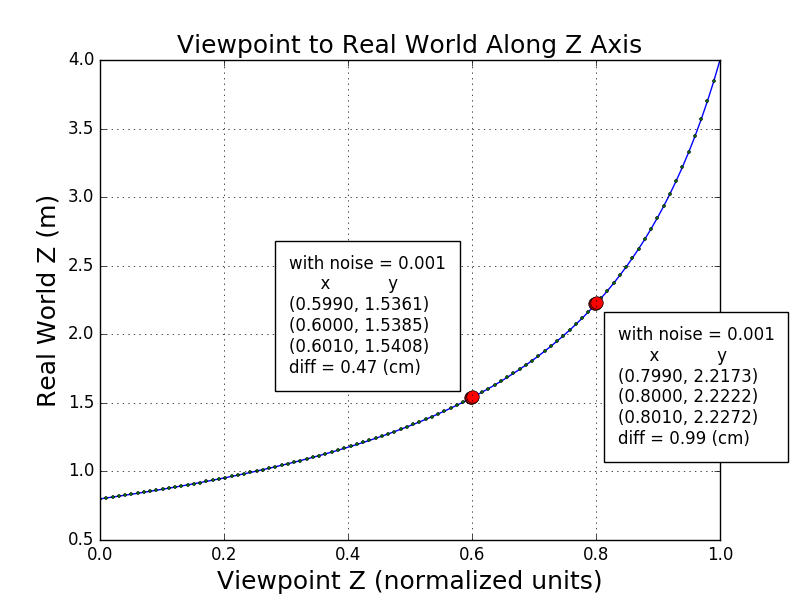
\includegraphics[width=.5\textwidth]{figures/plot_depth.png}
\caption{Viewpoint coordinates to real world coordinates analysis. Viewpoint coordinates are obtained when a mesh is rendered into a render window, and can be transformed to real-world coordinates using the transformation matrix of the camera. Noise is added in simulation to the viewpoint coordinates. This graph shows the effect of that noise in real-world coordinates.}
\label{fig:depth}
\end{figure}
